\documentclass[aspectratio=169]{beamer}

\beamertemplatenavigationsymbolsempty

\usepackage[utf8]{inputenc} % codificacao de caracteres
\usepackage[T1]{fontenc}    % codificacao de fontes
\usepackage[brazil]{babel}  % idioma
\usetheme{CambridgeUS}         % tema
\usecolortheme{dolphin}      % cores
\usefonttheme[onlymath]{serif} % fonte modo matematico
\usepackage{hyperref}

% Definindo novas cores
\definecolor{verde}{rgb}{0,0.5,0}
\definecolor{branco}{rgb}{1,1,1}
% Configurando layout para mostrar codigos C++
\usepackage{listings}
\lstset{
	language=C++,
	basicstyle=\ttfamily\scriptsize, 
	keywordstyle=\color{blue}, 
	stringstyle=\color{verde}, 
	commentstyle=\color{red}, 
	extendedchars=true, 
	showspaces=false, 
	showstringspaces=false, 
	numbers=left,
	numberstyle=\tiny,
	breaklines=true, 
	backgroundcolor=\color{green!10},
	breakautoindent=true, 
	captionpos=a,
	xleftmargin=0pt,
}

\usepackage{tikz}
\usetikzlibrary{automata,positioning}


\newcommand{\TITLE}{PROJETO DE UM SISTEMA OPERACIONAL}
\newcommand{\AUTHOR}{Samuel Felipe dos Santos}
\newcommand{\SUBJECT}{Apresentação 2 ponto de chegagem de Laboratório de Sistemas Operacionais 2016.}
\newcommand{\KEYWORDS}{Apresentação,
	Laboratório,
	Sistemas Operacionais}

\hypersetup{linkcolor = black,
	citecolor = black,
	filecolor = black,
	urlcolor = black,
	pdftitle = {\TITLE}, 
	pdfauthor = {\AUTHOR},
	pdfsubject = {\SUBJECT}, 
	pdfkeywords = {\KEYWORDS}
}





% Titulo
\title[\sc{PROJETO DE UM SISTEMA OPERACIONAL}]{\TITLE}
\author[\AUTHOR]{\AUTHOR}
\institute[ICT - UNIFESP]{Instituto de Ciência e Tecnologia\\Universidade Federal de São Paulo} % opcional
\date{\today}


\bibliographystyle{apalike}


\begin{document}
	
	\begin{frame}
		\titlepage
	\end{frame}
	
	\begin{frame}
		\tableofcontents
	\end{frame}
	
	
	\section{Introdução}
	\subsection{Motivação}
	\begin{frame}{Introdução}	
		\framesubtitle{Motivação}
		\begin{itemize}
			
			
			\item Para \textbf{facilitar} a interação entre o \textbf{usuário} e o \textbf{sistema} computação, existe um programa denominado \textbf{Sistema Operacional}.
			
			\vspace{0.5cm}
			
			\item O Sistema Operacional tem três principais objetivos:
			
			\begin{itemize}
					 
				\item \textbf{Executar programas} do usuário e solucionar seus problemas; 
				
				\vspace{0.2cm}
				
				\item Tornar o uso do Sistema Computacional \textbf{Conveniente}; 
				
				\vspace{0.2cm}
				
				\item Utilizar o \textbf{hardware} do computador de maneira \textbf{eficiente}.
			
			\end{itemize}		
			
		\end{itemize}
	\end{frame}


\setbeamercolor{block title}{bg=structure.fg!20!bg!50!bg}

	\subsection{Objetivos}
	\begin{frame}
		\frametitle{Introdução}	
		\framesubtitle{Objetivos}
		
		  \begin{block}{Objetivos Gerias}
		  			  		
			  	\textbf{Implementaç\~ao de um sistema operacional} capaz de gerenciar processos, memória e unidades de entrada e saída;
			  	
			  	\vspace{0.5cm}
		  	
			  	Linhagem de programação \textbf{C-};
			  	
			  	
			  	\vspace{0.2cm}
			  	
			  	\textbf{Compilador} para \textbf{traduzi-lo} para o conjunto de instruções do sistema computacional;
			
		  \end{block}
		  
		  \vspace{0.5cm}
		  
		  \begin{block}{Objetivos Específicos}
			  Definição do Sistema Operacional a ser projetado;
			  
			  \vspace{0.5cm}
			  
			  Definição das técnicas e algoritmos a serem virtualizados;
		  \end{block}
		
		
	\end{frame}

		

	\section{Fundamentação Teórica}
	\begin{frame}{Fundamentação Teórica}
		
		Conceitos importantes para o desenvolvimento do projeto:
		
		\vspace{0.5cm}
		
		\begin{itemize}
			\item CPU;
			
			\vspace{0.5cm}
			
			\item Compilador;
			
			\vspace{0.5cm}
			
			\item Sistemas Operacionais.
		\end{itemize}
	\end{frame}
	
	
	\subsection{CPU}
	\begin{frame}{CPU}
			
		\only<1>{
			\begin{itemize}
				\item CPU (Central Processing Unit), ou UCP (Unidade Central de
				Processamento);
				
				\vspace{0.5cm}
					
				\item Realiza \textbf{cálculos} e \textbf{operações} de acordo com um \textbf{programa};
				
				\vspace{0.5cm}
				
				\item Pode ser dividido em Unidade de Processamento e Unidade de Controle.
				\begin{itemize}
					\item \textbf{Unidade de Processamento:} local onde o processamento ocorre;
					
					\vspace{0.2cm}
					
					\item \textbf{Unidade de Controle:} Tem a função de \textbf{controlar} as diversas \textbf{unidades} que compõem a Unidade de Processamento .
				\end{itemize}
				
			\end{itemize}
			
		}
	
	\end{frame}
	
	\subsection{Compilador}	
	\begin{frame}{Compilador}	
		
		\only<1>{
			\begin{itemize}
				\item Traduz um programa escrito em uma \textbf{linguagem fonte} para uma linguagem \textbf{alvo};
				
				\vspace{0.5cm}
				
				\item Relata a presença de \textbf{erros} no código fonte; 
				
				\vspace{0.5cm}
				
				\item Pode ser dividido em:
				
				\begin{itemize}
					\item Análise Léxica;
					
					\vspace{0.2cm}
					
					\item Análise Sintática;
					
					\vspace{0.2cm}
					
					\item Análise Semântica;
					
					\vspace{0.2cm}
					
					\item Geração de Código Intermediário;
					
					\vspace{0.2cm}
					
					\item Otimização;
					
					\vspace{0.2cm}
					
					\item Geração de Código Objeto.
					 
				\end{itemize}
			\end{itemize}
			
			
		}

	\end{frame}
	
	\subsection{Sistema Operacional}
	\begin{frame}{Sistema Operacional}	
		\begin{itemize}
			
			
			\item \textbf{Intermediário} entre o usuário e o hardware de um computador;
			
			\vspace{0.5cm}
			
			\item Funcionalidades que podem ser destacadas:
			
			\begin{itemize}
				\item Escalonamento da CPU;
				
				\vspace{0.2cm}
				
				\item Gerenciamento de Memória;
				
				\vspace{0.2cm}
				
				\item Gerenciamento de Entrada e Saída. 
			\end{itemize}
					
		\end{itemize}

	\end{frame}
	
	
	\section{O Projeto}
	\begin{frame}{O Projeto}
		
		O projeto é dividido em três componentes:
		\begin{itemize}
			\item O Processador;
			
			\vspace{0.2cm}
			
			\item O Compilador;
			
			\vspace{0.2cm}
			
			\item O Sistema Operacional.
		\end{itemize}
	
	\end{frame}

	\subsection{O Processador} 
	\begin{frame}{O Processador}
		\only<1>
		{
			\framesubtitle{Definições Gerais}
			\begin{itemize}
				\item 32 bits;
			
			\vspace{0.5cm}
			
				\item Arquitetura Load/Store;
				
				\vspace{0.5cm}
				
				\item 28 instruções;
				
				
				\vspace{0.5cm}
				
				\item Monociclo.
			\end{itemize}
		}
		\only<2>
		{
			\framesubtitle{Diagrama da CPU}
			
			\begin{figure}
				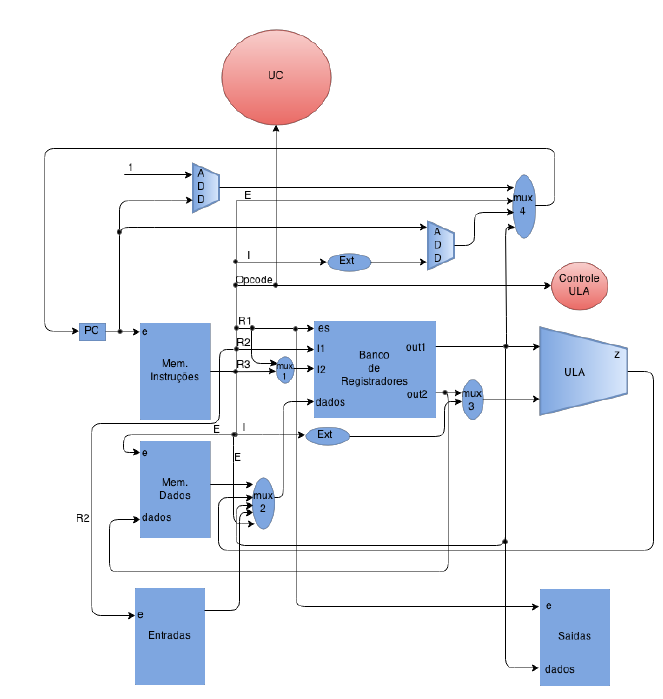
\includegraphics[height=0.8\textheight]{figuras/Diagrama_da_cpu}
				\caption{Diagrama da CPU}
			\end{figure}
				
		}
		\only<3>
		{
			\framesubtitle{Diagrama dos Sinais de Controle da CPU}
			
			\begin{figure}
				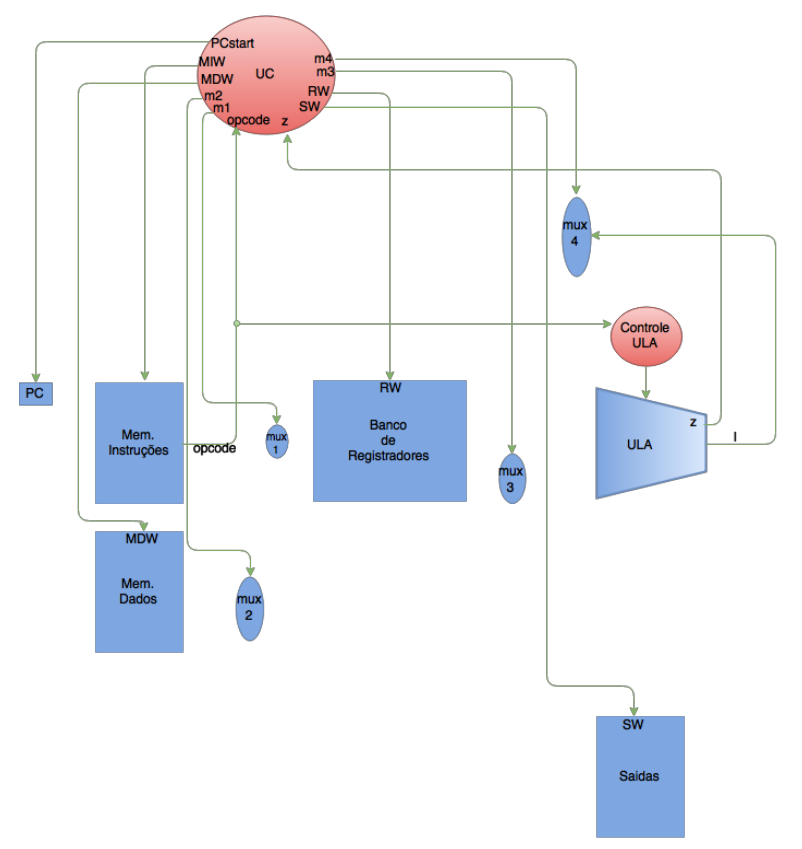
\includegraphics[height=0.8\textheight]{figuras/Diagrama_dos_sianais_de_comtrole_da_cpu}
				\caption{Diagrama dos Sinais de Controle da CPU}
			\end{figure}
			
		}
		
		
		
	\end{frame}
	
	\subsection{O Compilador}
	\begin{frame}{O Compilador}
		\only<1>
		{
			\framesubtitle{Definições Gerais}
			
			\begin{itemize}
				\item Lingagem de Programação: \textbf{C++};
				
				\vspace{0.5cm}
				
				\item Ferramentas: \textbf{Flex} e \textbf{Bison};
				
				\vspace{0.5cm}
				
				
				\item $C \to Instruções do Processador$
			\end{itemize}
			
		}
		\only<2>
		{
			\framesubtitle{A Linguagem C-}
			
			Diferenças em relação ao C:
			
			\begin{itemize}
				\item \textbf{Não} podem haver declarações de \textbf{protótipos de funções};
				
				\vspace{0.5cm}
				
				\item Apenas inteiros (\textbf{int});
				
				\vspace{0.5cm}
				
				\item \textbf{Não} há utilização de \textbf{ponteiros};
				
				\vspace{0.5cm}
				
				\item \textbf{Variáveis} declaradas no \textbf{inicio};
				
				
				\vspace{0.5cm}
				
				\item Funções \textbf{input} e \textbf{output}.
			\end{itemize} 
		}
		\only<3>
		{
			\framesubtitle{Erros Detectados}
			\begin{itemize}
				\item Atribuição de \textbf{variável a vetor} ou vetor a variável;
				
				\vspace{0.5cm}
				
				\item \textbf{Retorno} de função como vetor;
				
				\vspace{0.5cm}
				
				\item Criação de \textbf{variáveis} do tipo \textbf{void};
				
				\vspace{0.5cm}
				
				\item Utilização de variáveis \textbf{não declaradas}; 
				
				\vspace{0.5cm}
				
				\item Declaração de variáveis \textbf{já declaradas};
				
				\vspace{0.5cm}
				
				\item Programa \textbf{sem função main}.
			\end{itemize}
		}
	\end{frame}
	
	\subsection{O Sistema Operacional}
	\begin{frame}{O Sistema Operacional}
		\only<1>
		{
			O Sistema Operacional terá sua implementação dividida em \textbf{2 partes}:
			
			\begin{itemize}
				\item Mudanças em Hardware;
			
			\vspace{0.5cm}
			
				\item Implementação em Software.
			\end{itemize}
		}
		\only<2>
		{
			\framesubtitle{Mudanças em Hardware}
			\begin{itemize}
				
				\item Criação de \textbf{3 buffers} de propósito geral.
				
				\vspace{0.5cm}
				
				\item Intruções de acesso aos buffer: 
				\begin{itemize}
					\item push;
					\vspace{0.2cm}
					\item FIFOpop;
					\vspace{0.2cm}
					\item STACKpop;
					\vspace{0.2cm}
					\item write;
					\vspace{0.2cm}
					\item read;
					\vspace{0.2cm}
					\item top;
					\vspace{0.2cm}
					\item down; 
				\end{itemize}
			
			\end{itemize}			
		}
		\only<3>
		{
			\framesubtitle{Implementação em Software: Gerenciamento de Processos}
			\begin{itemize}
				
				\item Os processos serão constituídos dos seguintes componentes:
				
					\begin{itemize}
						\item \textbf{Instruções} contidas na memória de instruções;
					\vspace{0.5cm}
						\item \textbf{Zona na memória} de dados;
					\vspace{0.5cm}
						\item Um contador de programa (\textbf{PC}). 
					\end{itemize} 
				
			\end{itemize}
		}
		\only<4>
		{
			\framesubtitle{Implementação em Software: Gerenciamento de Processos}
			\begin{figure}[!htb]
				\centering
				\footnotesize
				\begin{tikzpicture}[shorten >=0.5pt,node distance=3.2cm,auto] 
				\node[state,initial] (q_0)   {Pronto}; 
				\node[state] (q_1) [right=of q_0] {{\tiny Executando}}; 
				\node[state] (q_2) [below left of= q_1] {{\tiny Bloqueado}}; 
				
				\path[->] 
				(q_0) edge[bend left] node[above]  {{\footnotesize processo escalonado}} (q_1)
				
				edge [loop above] node[align=left] {Outro processo\\ em execução} ()
				
				(q_1) edge [loop above] node[align=left] {Processo continua\\ em execução} ()
				
				edge[bend left] node[below]  {sofre preempção} (q_0)
				
				edge node {Processo esperando $I/O$} (q_2)
				
				(q_2)edge [loop below] node {Processo esperando $I/O$} ()
				
				edge node {$I/O$ resolvida} (q_0);
				
				
				\end{tikzpicture}
				
				\caption{Diagrama de Estados dos Processos}
				\label{fig::DiagramaProcessos}
			\end{figure}
			
		}
		\only<5>
		{
			\framesubtitle{Implementação em Software: Gerenciamento de Memória}
			\begin{itemize}
				
				\item \textbf{Multiprogramação com partições fixas};
				
				
				\vspace{0.5cm}
				
				\item Executado na \textbf{inicialização} do SO;
				\vspace{0.5cm}
				\item Partição de \textbf{tamanho variável};
				\vspace{0.5cm}
				\item Um processo sempre usa a \textbf{mesma partição}.
				
			\end{itemize}
		}
		\only<6>
		{
			\framesubtitle{Implementação em Software: Gerênciamento de Entrada e Saída}
			\begin{itemize}
				\item Disponibilizar acesso \textbf{assíncrono} aos dispositivos;
				\vspace{0.5cm}
				\item Faz uso dos \textbf{módulos} de Entrada e Saída;
				\vspace{0.5cm}
				\item \textbf{Move} processos entre a \textbf{fila de prontos} e a \textbf{fila de bloqueados};
			\end{itemize}
		}
	\end{frame}
	
	
	
	\section{Etapas Futuras e Possíveis Melhorias}
	\begin{frame}{Etapas Futuras e Possíveis Melhorias}
		Próxima etapa: a implementação no \textbf{FPGA} (Field Programmable Gate Array) Cyclone IV EP4CE115F29C7.
		\vspace{0.5cm}
		Possíveis melhorias que poderiam ser implementadas são:
		
			\begin{itemize}
				\item \textbf{Paginação} e \textbf{Segmentação da memória};
				\vspace{0.5cm}
				\item \textbf{Outros métodos} de escalonar processos;
				\vspace{0.5cm}
				\item Implementação de \textbf{interrupções}; 
				\vspace{0.5cm}
				\item Implementação de \textbf{comunicação entre processos};
				\vspace{0.5cm}
				\item Implementação de \textbf{DMA}.
			\end{itemize}
	\end{frame}
	
	
	
\end{document}